\documentclass[a4paper,11pt,oneside]{article}

\usepackage{amsmath,amssymb,epsfig}
\usepackage[T1]{fontenc}
\usepackage{ae,aecompl}
\usepackage{url}
\usepackage{subfigure}
\addtolength{\voffset}{-1cm}
\addtolength{\hoffset}{-1cm}
\setlength{\parindent}{0in}
\addtolength{\textwidth}{1.8cm}
\addtolength{\textheight}{1cm}
\addtolength{\parskip}{.5cm}

% Example definitions.
% --------------------
\def\e{{e^{j\omega}}}
\def\W{{W_M}}
\def\sumk{{\sum_{k=-\infty}^{\infty}}}
\def\x{{\mathbf x}}
\def\X{{\mathbf X}}
\def\Y{{\mathbf Y}}
\def\u{{\mathbf u}}
\def\U{{\mathbf U}}
\def\x{{\mathbf x}}
\def\s{{\mathbf s}}
\def\A{{\mathbf A}}
\def\y{{\mathbf y}}
\def\w{{\mathbf w}}
\def\B{{\mathbf B}}
\def\a{{\mathbf a}}
\def\D{{\mathbf D}}
\def\P{{\mathbf P}}
\def\n{{\mathbf n}}
\def\V{{\mathbf V}}
\def\R{{\mathbf R}}
\def\I{{\mathbf I}}
\def\M{{\mathbf M}}
\def\sech{{\mathrm{sech}}}
\def\L{{\cal L}}
\def\Cum{{\rm{Cum}}}
\def\var{{\rm{var}}}
\def\T{{\mathbf T}}
\def\C{{\mathbf C}}
\def\tf{{\emph{t-f}}}


% Title.
% ------
\title{SGN-1107 Introductory Signal Processing\\
Sample exam}
%
% Author and date.
% ---------------
\date{\today}
\author{Germ\'an G\'omez-Herrero, \url{http://germangh.com}}



\begin{document}

\maketitle


\textbf{QUESTION 1 (3 points):}  Consider a system with the following input-output relationship:

\[
y[n] = \frac{1}{x[n]}+x[n-1]
\]

where $x[n]$ is the input to the system and $y[n]$ is the system's output. Is this system linear? (1 point) Is it time-invariant? (1 point). Could you determine the ouput of the system to an arbitrary input by using only the system's impulse response? (1 point). Justify your answers. 

\vspace{1cm}

\textbf{SOLUTION:}

\textbf{Is the system linear?}

Consider the input sequence $a[n]=\alpha x_1[n]+\beta x_2[n]$ with $\alpha$ and $\beta$ being two arbitrary scalar and $x_1[n]$ and $x_2[n]$ being two arbitrary sequences. Then, if the system is linear, it must be satisfy that the output to $a[n]$ is $y_a[n]=\alpha y_1[n] + \beta y_2[n]$ where $y_1[n]$ and $y_2[n]$ are the outputs of the system to the inputs $x_1[n]$ and $x_2[n]$, respectively. We can easily check that this system does not satisfy this condition and therefore the system is NOT linear:

\[
\begin{array}{lll}
y_a[n]&=&\frac{1}{\alpha\cdot x_1[n]+\beta\cdot x_2[n]}+\alpha\cdot x_1[n-1]+\beta\cdot x_2[n-1]\\ &\neq&\alpha\cdot\underbrace{\left(\frac{1}{x_1[n]}+x_1[n-1]\right)}_{y_1[n]}+\beta\cdot\underbrace{\left(\frac{1}{x_2[n]}+x_2[n-1]\right)}_{y_2[n]}
\end{array}
\]

\textbf{Is the system time-invariant?}

The system will be time invariant if a delayed input $x[n-\tau]$ produces a delayed output $y[n-\tau]$. Let us denote by $y_\tau[n]$ the output produced by $x[n-\tau]$. Then we can easily check that:

\[
y_\tau[n] = \frac{1}{x[n-\tau]}+x[n-1-\tau] =y[n-\tau]
\]

so the system is time-invariant.

\textbf{Is the system's impulse response enough for determining the output of the system to an arbitrary input?}

No. It would be enough only if the system would be linear and time-invariant (LTI) but this system is not linear. 


\vspace{1cm}

\textbf{QUESTION 2 (5 points):} Consider the discrete-time sequence:

\[
x[n] = \cos\left(\frac{n\pi}{5}\right)
\]

Find two different continuous-time signals $x(t)$ that would produce this sequence when sampled at a frequency of $f_s=10Hz$ (Hint: consider the cases of sampling above and below the Nyquist rate). 


\vspace{1cm}

\textbf{SOLUTION:}

\emph{This exercise is solved in the same way as question number 2 from the second toy exam available in the course web-page.}

Clearly, the given sequence is equivalent to these other sequences:

\[
x[n] = \cos\left(n\frac{\pi}{5}\right)= \cos\left(n\omega_0\right)=\cos\left(n(\omega_0+2\pi \cdot k)\right)=\cos(n\omega_k)
\]

where $k$ is any integer, i.e. $k=0, \pm 1, \pm 2,...$. The discrete-time angular frequencies $\omega_k=\omega_0+2\pi \cdot k$ correspond to the following continuous-time frequencies:

\[
\Omega_k = \omega_k \cdot f_s = \left(\frac{\pi}{5}+2\pi \cdot k\right)\cdot 10
\]

Taking different values of $k$ we can obtain different continuous-time signals that will produce the same discrete-time sequence. For instance:

\[
\begin{array}{lllll}
k = 0 &\Rightarrow& \Omega_0 = \frac{\pi}{5}\cdot 10 &\Rightarrow& x_0(t)=\cos(\frac{\pi}{2}t)\\
k = 1 &\Rightarrow& \Omega_1 = (\frac{\pi}{5}+2\pi)\cdot 10 &\Rightarrow& x_1(t)=\cos(\frac{41\pi}{2}t)\\
\end{array}
\]


\vspace{1cm}

\textbf{QUESTION 3 (6 points):} Diagrammed below is a hybrid digital-analog system:

\begin{figure}[h!]
\centering
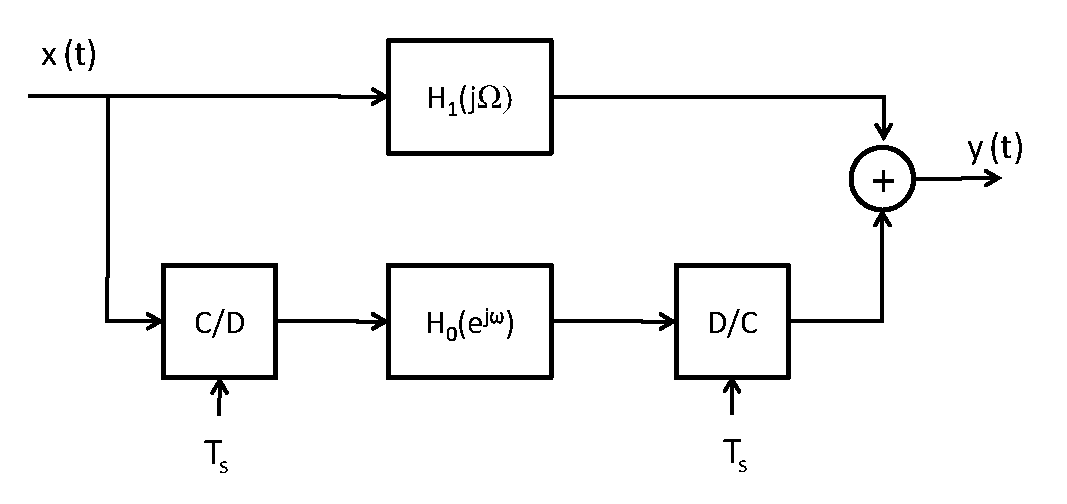
\includegraphics[width=.8\textwidth]{fig1.eps}
\label{fig1}
\end{figure} 

The discrete-time system is a filter with a frequency response $H_{0}(e^{j\omega})$, which has the following shape:

\begin{figure}[h!]
\centering
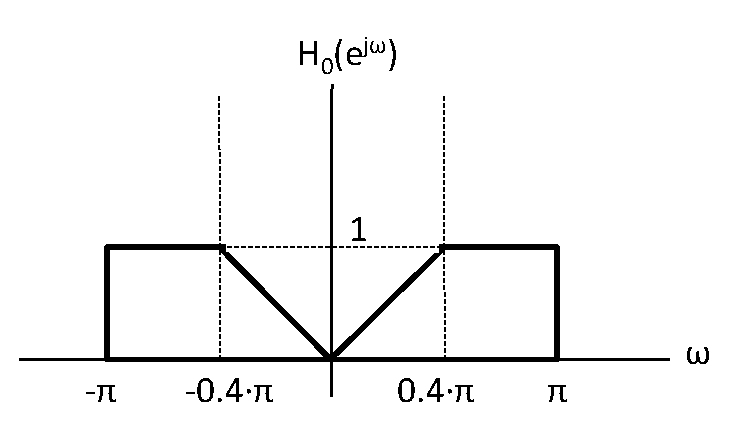
\includegraphics[width=.5\textwidth]{fig2.eps}
\label{fig2}
\end{figure} 

The input baseband analog signal is bandlimited to $\Omega_{max}=2\pi\cdot 4000$, and the sampling period of the ideal C/D and D/C converters is $T_s=10^{-4}\; s$. Depict the shape that the analog system $H_{1}(j\Omega)$ must have in order to obtain perfect reconstruction, i.e. $y(t)=x(t)$ (2 points). Specify the numeric value of the relevant frequencies where the shape of $H_{1}(j\Omega)$ changes and the amplitude of $H_{1}(j\Omega)$ at those relevant frequencies (4 points). 


\vspace{1cm}

\textbf{SOLUTION:}

\emph{This problem is almost identical to question 4 from exercise 3, which is available at the course web-page}.

We can easily check that the sampling period of the system $T_s=10^{-4}$ seconds is small enough so that aliasing is avoided for all $|\Omega|<2\pi\cdot 4000=\Omega_{max}$. That is, the sampling period of the system is smaller than the sampling period corresponding to the Nyquist rate:

\[
T_{Nyquist} = \frac{2\pi}{\Omega_{Nyquist}}=\frac{2\pi}{2\cdot\Omega_{max}}=\frac{2\pi}{2\cdot 2\pi \cdot 4000}=\frac{1}{8}\cdot 10^{-3}\;\textrm{seconds}
\]

whis is larger than $T_s=10^{-4}$. Then, the lower branch of the system (consisting of the two converters and the digital filter) is equivalent to an analog filter with frequency response:

\[
H_0(j\Omega)=H_0(e^{j\omega})|_{w=\Omega\cdot T_{s}}
\]

That is, the frequency response of the equivalent analog filter $H_{0}(j\Omega)$ is the result of de-normalizing $H_{0}(e^{j\omega})$ using the transformation $\Omega=\frac{\omega}{T_s}$:

\begin{figure}[h!]
\centering
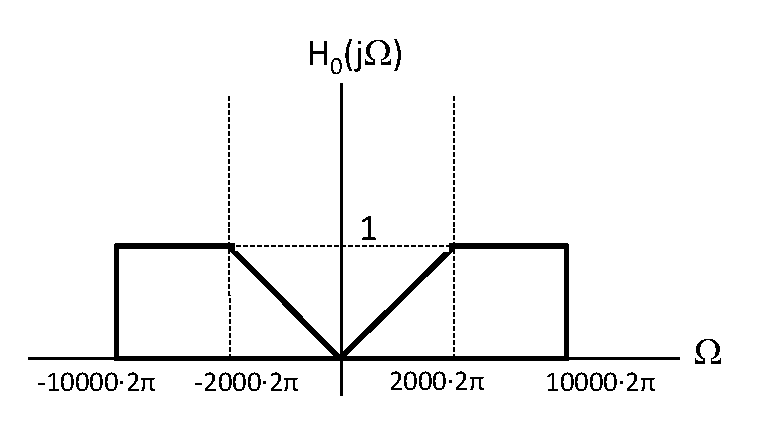
\includegraphics[width=.5\textwidth]{fig3b.eps}
\label{fig3b}
\end{figure} 

So the input-ouput relationship in Fourier domain is: 

\[
Y(j\Omega)=X(j\Omega)\cdot H_{0}(j\Omega)+X(j\Omega)\cdot H_1(j\Omega)=X(j\Omega)\cdot\left[H_{0}(j\Omega)+H_{1}(j\Omega)\right]
\]

For perfect reconstruction we need that:

\[
Y(j\Omega)=X(j\Omega)\Rightarrow H_{0}(j\Omega)+H_{1}(j\Omega)=1 \Rightarrow H_1(j\Omega)=1-H_0(j\Omega)
\]

for all $|\Omega|<\Omega_{max}=2\pi\cdot 4000$. So we have finally obtained that the analog filter $H_{1}(j\Omega)$ must have the following shape:


\begin{figure}[h!]
\centering
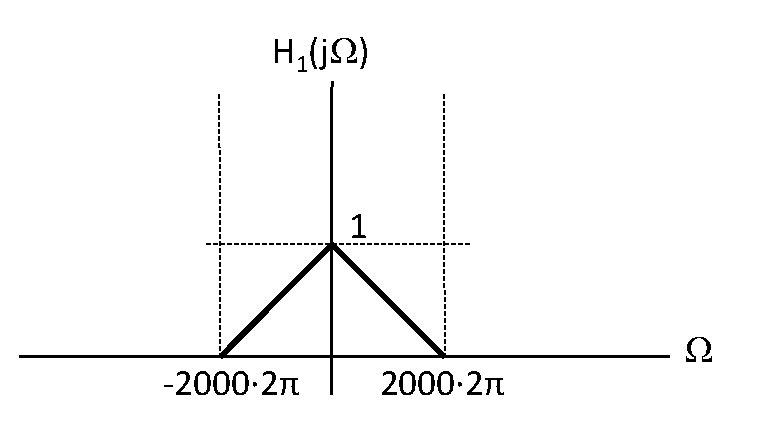
\includegraphics[width=.5\textwidth]{fig3c.eps}
\label{fig3b}
\end{figure} 

\vspace{3cm}

\textbf{QUESTION 4 (6 points):} Consider the system shown below. Assume that the input is bandlimited, $X_a(j\Omega)=0$ for $|\Omega|>2\pi\cdot 1000$.

\begin{figure}[h!]
\centering
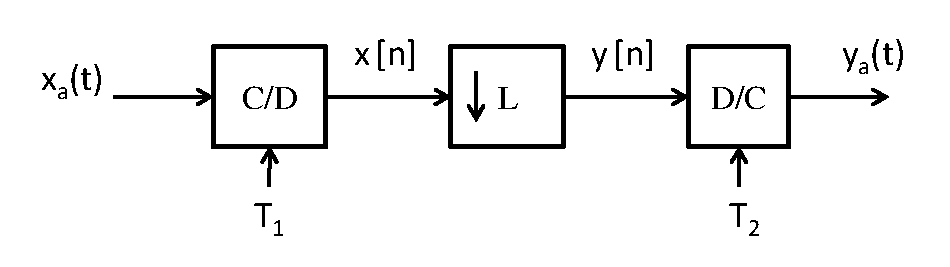
\includegraphics[width=.8\textwidth]{fig3.eps}
\label{fig3}
\end{figure} 
\begin{itemize}
\item[(a)] (3 points) What constraints must be placed on $L$, $T_1$, and $T_{2}$ in order for $y_a(t)$ to be equal to $x_a(t)$? Sketch the Fourier transforms of $x_a(t)$, $x(n)$, $y(n)$, and $y_a(t)$.
\item[(b)] If $f_1=f_2=20kHz$ and $L=4$, find an expression for $y_a(t)$ in terms of $x_a(t)$ (2 points). What is the energy of $y_{a}(t)$ with respect to the energy of $x_{a}(t)$ (1 point)?
\end{itemize}

\vspace{1cm}

\textbf{SOLUTION:}

\emph{This question is identical to question 3 from homework 4, which is available at the course web-page. This problem is solved with great level of detail only for teaching purposes. In the exam you should show ONLY the major intermediate steps and skip unnecessary explanations.}

\textbf{(a)}


Without loss of generality, in the following we will assume that the CTFT of the input analog signal $x_a(t)$ looks like depicted in Fig.~\ref{ctftxa}.

\begin{figure}[h!]
\centering
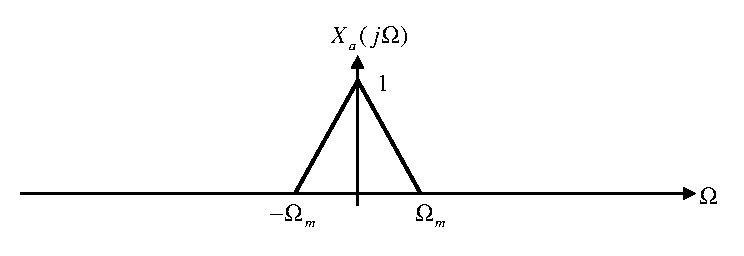
\includegraphics[width=.8\textwidth]{ctftxa.eps}
\caption{CTFT of the input analog signal $x_a(t)$.}
\label{ctftxa}
\end{figure}


where $\Omega_{m}=2\pi\cdot 1000$ is the maximum frequency present in $x_a(t)$. For perfect reconstruction to be possible, aliasing in the C/D transformation must be avoided. So the first contraint that has to be fullfiled is:

\begin{equation}\label{const1}
\Omega_1=\frac{2\pi}{T_1}\geq 2\Omega_{m} \Rightarrow T_1\leq  \frac{2\pi}{2\Omega_{m}}=\frac{2\pi}{2\cdot 2\pi\cdot 1000}\Rightarrow T_1\leq 5\cdot 10^{-4} \;\textrm{seconds}
\end{equation}

Remember that in the D/C block take place two subsequent operations. First the input analog signal is multiplied by continuous-time train of impulses having an inter-impulse distance of $T_1$ seconds. The result is also a continuous time signal $x_s(t)$ which is non-zero only in those time instants that are an integer multiple of $T_1$:

\[
x_s(t)=\left\{ 
\begin{array}{lll}
x(t) &\qquad & \textrm{if}\; \frac{t}{T_1}\in\mathbb{Z}\\
0 & \qquad & \textrm{otherwise}
\end{array}
\right.
\]

The CTFT of $x_s(t)$ is depicted in Fig.~\ref{ctftxs}, where $\Delta=\Omega_1-2\Omega_m$ is the spacing between correlative copies of the spectrum of $x_a(t)$. Because we have enforced that $\Omega_1\geq 2\Omega_m$, it is obvious that $\Delta\geq 0$ and therefore there is overlap between two correlative spectral aliases, i.e. there is not aliasing.

\begin{figure}[h!]
\centering
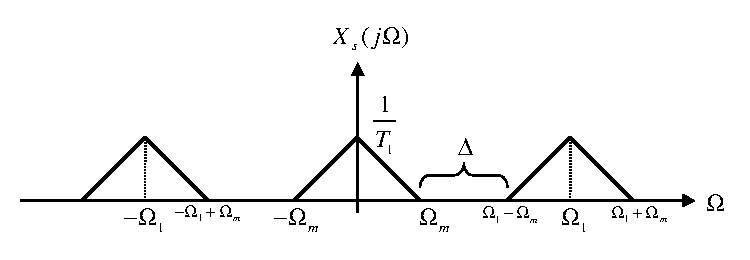
\includegraphics[width=.8\textwidth]{ctftxs.eps}
\caption{CTFT of the continuous-time sampled signal $x_s(t)$.}
\label{ctftxs}
\end{figure}

The DTFT $X(e^{j\omega})$ of the discrete-time signal $x[n]$ has the shape depicted in Fig.~\ref{ctftxs} but with the frequency normalization $\omega=\Omega\cdot T_1=\frac{\Omega\cdot 2\pi}{\Omega_1}$. This DTFT is depicted in Fig.~\ref{dtftx}.

\begin{figure}[h!]
\centering
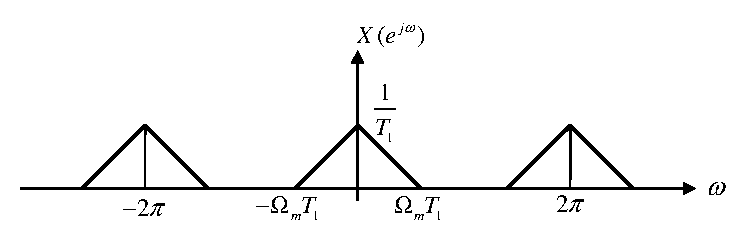
\includegraphics[width=.8\textwidth]{dtftx.eps}
\caption{DTFT of the discrete-time sequence $x[n]$.}
\label{dtftx}
\end{figure}

After the downsampler, the DTFT $Y(e^{j\omega})$ of the sequence $y[n]$ will be the obtained by expanding the frequency range $[-\pi,\pi)$ in Fig.~\ref{dtftx} and replicating the result every $2\pi$. This is depicted in Fig.~\ref{dtfty}.


\begin{figure}[h!]
\centering
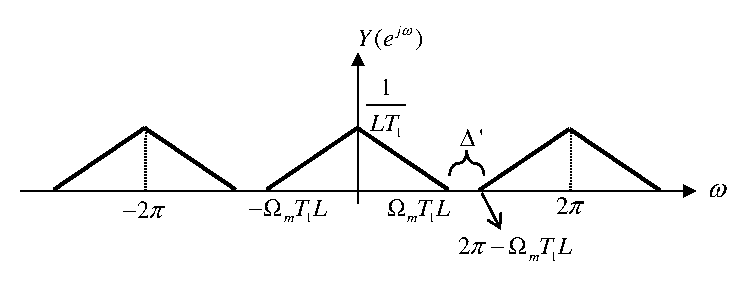
\includegraphics[width=.8\textwidth]{dtfty.eps}
\caption{DTFT of the discrete-time sequence $y[n]$.}
\label{dtfty}
\end{figure}

From Fig.~\ref{dtfty}, it is obvious that for perfect reconstruction to be possible, the space between correlative spectral aliases must be greater than 0, i.e:

\begin{equation}\label{const2}
\Delta'\geq 0 \Rightarrow 2\pi-2\Omega_mT_1L\geq 0 \Rightarrow T_1 \leq \frac{2\pi}{2\Omega_m L} \Rightarrow T_{1} \leq \frac{5\cdot 10^{-4}}{L} \; \textrm{seconds}
\end{equation}

Because $L\geq 2$, the constraint given by Eq.~\ref{const2} is more restrictive that the one found in Eq.~\ref{const1}. Therefore our new constraint for $T_1$ will be the one in Eq.~\ref{const2}.

The D/C block consists of two consecutive operations. First, the input discrete-time sequence $y[n]$ is converted into a continous-time signal $y_s(t)$, which is later passed through an ideal low-pass reconstruction filter with cutoff frequency $\frac{\Omega_m}{2}$ and gain $T_2$ to build the output analog signal $y_a(t)$. The purpose of the reconstruction filter is to extract the baseband signal and remove the other spectral aliases. The CTFT $Y_s(j\Omega)$ of $y_s(t)$ is depicted in Fig.~\ref{ctftys}. Clearly, for the reconstruction filter to output a copy of $x_{a}(t)$ the sampling period in the D/C block has to fulfil the constraint: 

\begin{equation}\label{const3}
T_2=T_1\cdot L
\end{equation}

If the condition above is fulfilled then the reconstruction filter will just retain the baseband component in $Y_s(j\Omega)$ and will amplify it by a factor equal to $T_2=L\cdot T_1$. Thus the CTFT of $y_a(t)$ will be the same as the CTFT of $x_a(t)$ and, therefore, $y_a(t)=x_a(t)$. Summarizing, the constraints in Eq.~\ref{const2} and Eq.~\ref{const3} have to be fulfilled for perfect reconstruction to occur.

\begin{figure}[h!]
\centering
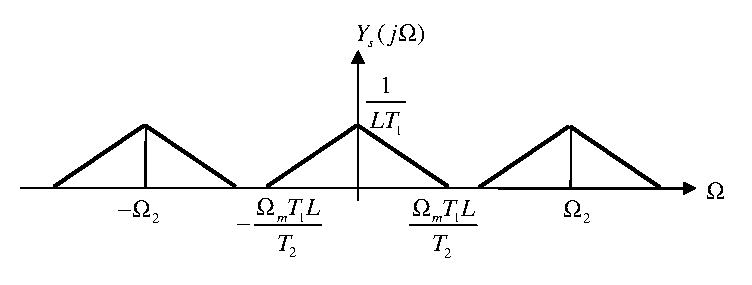
\includegraphics[width=.8\textwidth]{ctftys.eps}
\caption{CTFT of the continous-time signal $y_s(t)$. Notice that this is just the result of de-normalizing the frequencies in Fig.~\ref{dtfty} ($\Omega=\frac{\omega}{T_2}$).}
\label{ctftys}
\end{figure}


\vspace{1cm}
\textbf{(b)}

Since $f_1=f_2=f=2\cdot 10^4$ Hz, the sampling period in both the C/D and D/C blocks will be $T_1=T_2=\frac{1}{f}=5\cdot 10^{-5}$ seconds and their angular sampling frequencies will be $\Omega_s=2\pi f_s=4\cdot 10^{4}\pi$ radians/second. We can see that this sampling period fulfills the constraint in Eq.~\ref{const2}:

\[
T=5\cdot 10^{-5}<\frac{5\cdot 10^{-4}}{L}=\frac{5\cdot 10^{-4}}{4}=12.5\cdot 10^{-5}
\]

Therefore, neither the C/D block nor the downsampler will cause aliasing and the spectral aliases in Fig.~\ref{ctftys} will not overlap each other. In this case, the reconstruction filter will have a cutoff $\frac{\Omega_s}{2}=2\cdot 10^{4}\pi$ radians/seconds so that only the baseband alias in $Y_s(j\Omega)$ is retained. The CTFT of the output analog signal $y_a(t)$ is given in Fig.~\ref{ctfty}. 

\begin{figure}[h!]
\centering
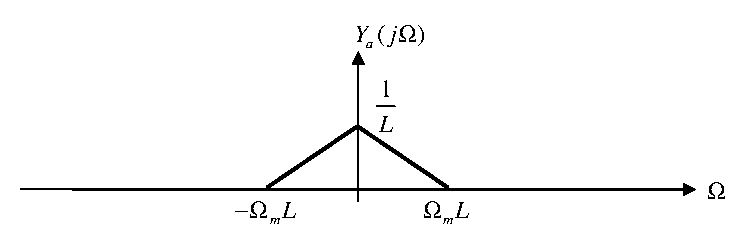
\includegraphics[width=.8\textwidth]{ctfty.eps}
\caption{CTFT of the continous-time output signal $y_a(t)$. Notice that this is just the result of making that $T_1=T_2=T$ in Fig.~\ref{ctftys} and applying a lowpass reconstruction filter with cutoff $\frac{\Omega_s}{2}$ and gain $T$.}
\label{ctfty}
\end{figure}

From Fig.~\ref{ctfty} we can see that the relationship between $Y_a(j\Omega)$ and $X_a(j\Omega)$ is:

\begin{equation}\label{relfreq}
Y_a(j\Omega) = \frac{1}{L}X_{a}(\frac{j\Omega}{L})=\frac{1}{4}X_{a}(\frac{j\Omega}{4})
\end{equation}

So the relationship in time domain is:

\begin{equation}
y_a(t)=x_a(Lt)=x_a(4t)
\end{equation}

Then the energy of the output analog signal is (by using Parseval's relation):

\begin{equation}\label{eqenergy}
E_{y_a}=\int_{-\infty}^{\infty}|y_a(t)|^2dt=\frac{1}{2\pi}\int_{-\Omega_mL}^{\Omega_mL}|Y_a(j\Omega)|^2d\Omega
\end{equation}

so using Eq.~\ref{relfreq} we have that:

\begin{equation}\label{energyfreq}
E_{y_a}=\frac{1}{2\pi}\int_{-\Omega_mL}^{\Omega_mL}|\frac{1}{4}X_a(\frac{j\Omega}{4})|^2d\Omega=\frac{1}{16}\cdot\frac{1}{2\pi}\int_{-\Omega_mL}^{\Omega_mL}|X_a(\frac{j\Omega}{4})|^2d\Omega
\end{equation}

and then by making the variable change $\Omega'=\frac{\Omega}{4}$ we have that $d\Omega=4d\Omega'$ and then Eq.~\ref{energyfreq} becomes:

\begin{equation}
E_{y_a}= \frac{4}{16}\cdot\frac{1}{2\pi}\int_{-\Omega_mL}^{\Omega_mL}|X_a(j\Omega')|^2d\Omega'=\frac{1}{4}E_{x_a}
\end{equation}

so the energy of the output signal is one fourth of the energy of the input signal.

The energy of the output could also have been obtained using the time-domain relationship between $y_a(t)$ and $x_a(t)$:

\begin{equation}\label{eqenergytime}
E_{y_a}=\int_{-\infty}^{\infty}|y_a(t)|^2dt=\int_{-\infty}^{\infty}|x_a(4t)|^2dt
\end{equation}

by making the variable change $m=4t$ we have that $dt=\frac{1}{4}dm$ and therefore, Eq.~\ref{eqenergytime} becomes:


\begin{equation}
E_{y_a}=\frac{1}{4}\int_{-\infty}^{\infty}|x_a(m)|^2dm=\frac{1}{4}E_{x_a}
\end{equation}

obtaining the same result that the energy of the ouput is one fourth of the energy of the input.


\vspace{1cm}

\textbf{QUESTION 5 (5 points):} Evaluate the convolution of the two sequences $h[n]=(0.5)^n\mu[n]$ and $x[n]=3^n\mu[-n]$ by using the Z-transform.


\vspace{1cm}

\textbf{SOLUTION:}

\emph{This question is identical to question 4 from the sample exam that was solved in the classroom and that is available in the course web-page.}

Using either the table of elementary Z-transform pairs or applying the formula of the foward Z-transform we obtain that:

\[
H(z) = \frac{1}{1-0.5z^{-1}} \qquad \textrm{ROC} \;\equiv\; |z|>0.5
\]

\[
X(z) = 1 - \frac{1}{1-3z^{-1}} \qquad \textrm{ROC} \;\equiv\; |z|<3
\]

So the Z-transform of the convolution $y[n]=x[n]\otimes h[n]$ is:

\[
Y(z)=X(z)H(z)=\frac{1}{1-0.5z^{-1}}-\frac{1}{(1-3z^{-1})(1-0.5z^{-1})} \qquad \textrm{ROC} \;\equiv\; 3>|z|>0.5
\]

the second fraction above can be expanded using the method of the residuals:

\[
\frac{1}{(1-3z^{-1})(1-0.5z^{-1})}=\frac{\frac{6}{5}}{1-3z^{-1}}-\frac{\frac{1}{5}}{1-0.5z^{-1}}
\]

so that we can write:

\[
Y(z)=\frac{1}{1-0.5z^{-1}}-\frac{\frac{6}{5}}{1-3z^{-1}}+\frac{\frac{1}{5}}{1-0.5z^{-1}}
\]

which can be directly inverted using the table of elementary Z-transform pairs:

\[
y[n] = \left(\frac{1}{2}\right)^{n}\mu[n]+\frac{6}{5}\left(3\right)^{n}\mu[-n-1]+\frac{1}{5}\left(\frac{1}{2}\right)^n\mu[n]
\]


\emph{The expression above is different to the expression that you can find in the solutions of the sample exam that we solved in the classroom. However, you can easily check that the expression there and here are equivalent.}

\vspace{1cm}

\textbf{QUESTION 6 (5 points):} Find the inverse Z-transform of

\[
X(z) = \frac{1-3z^{-5}}{(1-0.2z^{-1})(1+0.6z^{-1})} \qquad \textrm{ROC}\;\equiv\; 0.2<|z|<0.6
\]

\vspace{1cm}

\textbf{SOLUTION:}

Since the order of the numerator is greater that the order of the denominator we cannot apply directly the method of the residuals to $X(z)$. One way of proceeding is to perform a long division but this can be a rather long process. Since the numerator of our Z expression has only two terms the best is to rewrite $X(z)$ as:

\[
X(z)=\underbrace{\frac{1}{(1-0.2z^{-1})(1+0.6z^{-1})}}_{G(z)}-3z^{-5}\underbrace{\frac{1}{(1-0.2z^{-1})(1+0.6z^{-1})}}_{G(z)}
\]

and use the linearity and shifting properties of the Z-transform to write:

\[
x[n] = g[n] - 3g[n-5]
\]

where $g[n]$ is the inverse Z-transform of $G(z)$. Inverting $G(z)$ is very easy using the method of the residuals:

\[
G(z) = \frac{1}{(1-0.2z^{-1})(1+0.6z^{-1})}=\frac{\frac{1}{4}}{1-0.2z^{-1}}+\frac{\frac{3}{4}}{1+0.6z^{-1}}
\]

So we have that:

\[
g[n]=\frac{1}{4}(0.2)^n \mu[n]-\frac{3}{4}(-0.6)^n\mu[-n-1]
\]

and then $x[n] = g[n] - 3g[n-5]$.


\end{document}